\documentclass[11pt]{article}
\usepackage[a4paper,margin=1in]{geometry}
\usepackage[T1]{fontenc}
\usepackage{lmodern}
\usepackage{amsmath,amssymb}
\usepackage{booktabs}
\usepackage{graphicx}
\usepackage{xcolor}
\usepackage[numbers,sort&compress]{natbib}
\usepackage{caption}
\usepackage{microtype}
\usepackage{url}
\usepackage[colorlinks=true,linkcolor=blue!60!black,citecolor=blue!60!black,urlcolor=blue!60!black]{hyperref}
\captionsetup{font=small,labelfont=bf}
\graphicspath{{figures/}}
\newcommand{\J}{\ensuremath{J}}
\newcommand{\pending}[1]{\textcolor{red!70!black}{[#1]}}

\title{Model predictive pitch control with an agent-supervised learned residual:\\
\large the residual repairs the model, the agent supplies the reward's vocabulary}
\author{\pending{authors}}
\date{Preprint. \today}

\begin{document}
\maketitle

\begin{abstract}
Model predictive control (MPC) of wind-turbine pitch is only as good as its model, and reward design for a learned controller is only as good as its designer. We study the combination on collective-pitch control of the NREL~5\,MW turbine in OpenFAST: a linear-parameter-varying MPC whose cost is scaled correctly is the strongest controller on the metric set of a published RL pitch-control study (power MSE, generator-speed MSE, tower-base and blade-root fatigue), yet a 5\,\% error in its aerodynamic model halves its score and 15\,\% removes its advantage entirely. A bounded residual policy trained by PPO on top of the MPC, with a reward supervised every 30 episodes by a language-model agent under fork verification, adds about five points to the exact-model MPC on two disjoint held-out wind sets with every metric improved (tower fatigue reduction from 16 to 23--25\,\%), and restores the mismatched MPC from 4.5 to 13--18---above the exact-model MPC alone. A controlled study of the supervision itself, run with the same protocol on the residual's conventional base (the gain-scheduled PI), shows what the agent contributes: nothing through numeric levers (reward weights, hyper-parameters, where it ties random search), and, through the reward's expression, a vocabulary of term shapes that reaches a balanced solution no weight search reaches---which a random draw from the same vocabulary, verified by the same loop, reaches as well; the loop is necessary, the objective stated in the prompt is not, and the agent's effect on the level of the objective is within seed noise. We distil the findings into design rules: put learning where the model fails, put the agent on structure, verify against the true objective, one lever per agent, and report the composition of a solution alongside its mean.
\end{abstract}

\section{Introduction}

Above rated wind speed a turbine's collective pitch has to regulate rotor speed and power while limiting fatigue of the tower and the blades. Model predictive control (MPC) handles the trade-off explicitly and is a standard reference for this problem~\citep{Bossanyi2000,Soliman2011mpc,Koerber2013mpc,Schlipf2013nmpc,Evans2015rmpc}; reinforcement learning (RL) has been proposed as a model-free alternative~\citep{SierraGarcia2020,Xie2023rlpitch,Coquelet2022ipc,Baseline2026}. The two are usually compared, rarely combined, and the comparison hides two dependencies: the MPC depends on its model, and the RL controller depends on its reward. Language-model (LLM) agents now write and tune rewards---Eureka evolves reward code against a task score~\citep{Ma2024eureka}, Language-to-Rewards and Text2Reward map instructions to reward parameters and programs~\citep{Yu2023l2r,Xie2024text2reward}, DrEureka adds domain-randomisation design~\citep{Ma2024dreureka}, and agentic reward designers close the loop with semantic feedback~\citep{Lee2026rda}---which raises a third question: what does the agent actually contribute, beyond a search that any verification loop could run?

This paper answers the three questions on one benchmark with one protocol.

\paragraph{Does a learned residual add to a good model-based controller, and does it repair the model?} We put a bounded PPO residual on top of an LPV-MPC whose cost has been scaled so that its tower term works, and train it under a supervised reward. It adds about five points of the paper's metric-set objective to the exact-model MPC with every metric improved, and it restores an MPC whose aerodynamic model is 5\,\% off from 4.5 to 13--18---above the exact-model MPC alone (\S\ref{sec:main}).

\paragraph{What does the agent contribute to the residual's reward?} On the MPC base, about one point between a fixed and an agent-written reward. To see what that point is made of we run the supervision study on the residual's conventional base, the gain-scheduled PI, where the residual has more to do: three levers (reward weights, hyper-parameters, reward expression), each with a random-search control, plus loop ablations (\S\ref{sec:agent}). Numeric levers are worth nothing on a tuned default; the reward's shape is the one lever that changes what the solution is made of; the loop is necessary, the prompt's objective is not, and a random draw from the agent's own vocabulary of shapes does as well as the agent.

\paragraph{What is the reference conditional on?} The MPC's lead over every RL arm on the PI base is real but requires an exact aerodynamic model; a 5\,\% error on the power coefficient halves it (\S\ref{sec:mpc}). That fragility is the reason the residual has something to repair.

\paragraph{Contributions.}
(a)~The combination of a correctly scaled LPV-MPC with a supervised learned residual, evaluated on two disjoint held-out wind sets: $+5$ points over the exact-model MPC, every metric positive, and a 5\,\% model error repaired.
(b)~A controlled protocol for agentic supervision of a learning controller---three levers, random-search controls, seed pairing, exact permutation tests, tuned fixed defaults---and its outcome: the agent's contribution is a vocabulary of reward shapes made real by verification against the true objective, not the search and not the prompt.
(c)~A corrected model-based reference: the published verdict that MPC ``loses tower fatigue'' is a cost-scaling artefact; with $O(1)$ cost terms the same three-state MPC is positive on all four metrics, and its sensitivity to model error is quantified.

\section{Setup}

\subsection{Plant, reference controller, wind}
NREL~5\,MW onshore turbine~\citep{Jonkman2009nrel5mw} in OpenFAST~4.2.1~\citep{OpenFAST}, controlled by ROSCO~2.10.5~\citep{Abbas2022rosco} through a patched ZeroMQ interface at the 10\,ms control step. The ROSCO configuration is the gain-scheduled PI (GSPI) with peak shaving on and every other load-mitigation feature off, constant torque above rated; it is the pairing reference for every metric. Wind fields: TurbSim, 8, 12.5 and 15\,m/s mean hub wind, turbulence intensity 8\,\%, 150\,s episodes of which 130\,s are scored. Realisations with TurbSim seeds 1--2 are the supervisor's evaluation winds; seeds 3--6 and seeds 7--10 are two disjoint held-out sets (``wind seeds 3--6'' and ``wind seeds 7--10'' below). Fatigue is the damage-equivalent load from rainflow counting~\citep{fatpack,IEC61400}.

\subsection{Objective and statistics}
\label{sec:objective}
The objective is the metric set of \citep{Baseline2026} as one scalar,
\begin{equation}
\J = \tfrac14\!\sum_{m\in\{P,\omega,T,B\}}\!\mathrm{clip}_{\pm100}\big(\Delta m\,[\%]\big)\;-\;20\,\max\!\big(0,\;E_{\mathrm{loss}}[\%]-1\big),
\label{eq:J}
\end{equation}
the mean of the per-episode-clipped percentage reductions, relative to paired GSPI, of power MSE and generator-speed MSE on above-rated steps (labelled by hub wind, whatever the controller does) and of tower-base and blade-root fatigue, minus a penalty for energy loss beyond 1\,\%. Every selection (fork winner, best checkpoint, rollback) uses \J; every reported number is a held-out evaluation of the best checkpoint by the supervisor-side \J. Seeds are paired across arms; differences are reported as mean, wins$/n$, the exact two-sided sign-flip permutation $p$ (floor $2/2^n$: 0.0625 at $n=5$, 0.25 at $n=3$) and a paired $t$-test. Arms with $n=3$ are proofs of concept and are labelled as such.

\subsection{The model-based controller and what it is conditional on}
\label{sec:mpc}
A three-state LPV-MPC (rotor, first tower fore-aft mode) linearised every 0.1\,s from the $C_P$/$C_T$ tables, horizon 2\,s, OSQP~\citep{Stellato2020osqp} (3.6\,ms per solve), pitch within the live peak-shaving floor and the rate limit, wind held at ROSCO's low-passed estimate (no preview, unlike~\citep{Schlipf2013nmpc,Koerber2013mpc}), torque native. Its cost has three terms---speed error, tower-top velocity, pitch increment---each scaled to $O(1)$ at its typical value (Appendix~\ref{app:mpc}). The scaling matters: with the speed error normalised by rated speed instead, the speed term is $O(10^{-5})$ at a typical error of 0.5\,\% while the tower term is $O(1)$, any tower weight above zero out-weighs regulation by four orders of magnitude, and the optimum feathers the rotor---which reproduces the published verdict that MPC ``wins regulation and loses tower fatigue'' ($-17.6$\,\% here). With $O(1)$ terms and weights selected on wind seeds 1--2 by \J\ (the same rule as every learned arm), the MPC is positive on every metric: 12.4\,/\,14.1 on the two held-out sets with full pitch authority, 12.0\,/\,11.6 through the $\pm2.9^\circ$ damped residual channel the RL uses.

\begin{figure}[t]
\centering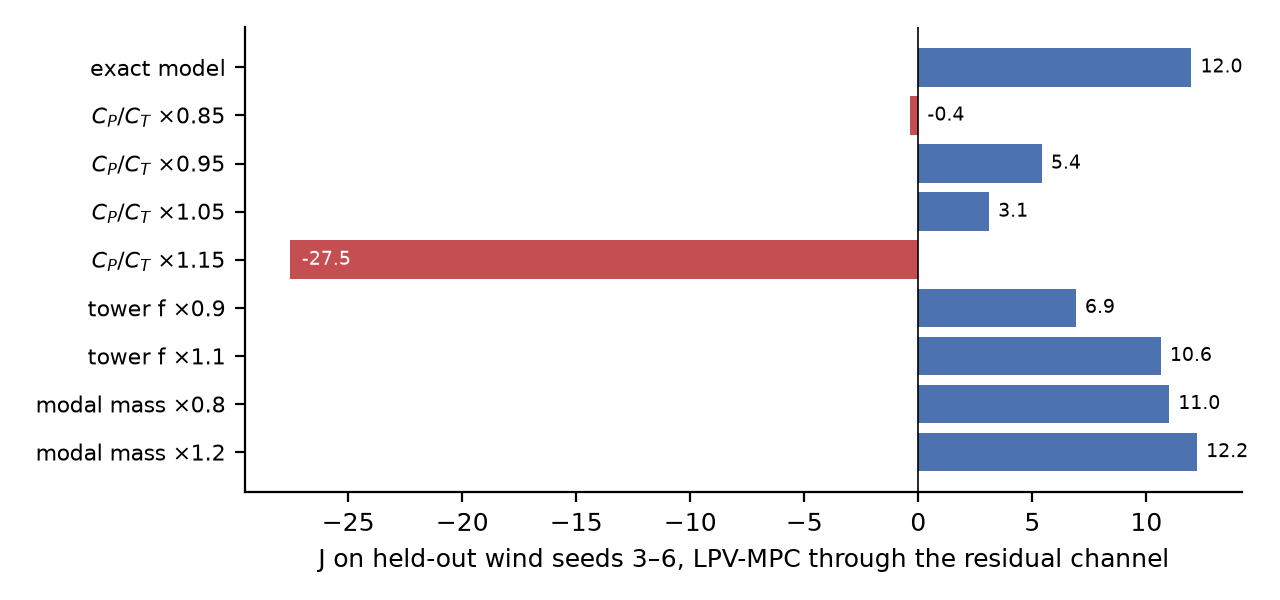
\includegraphics[width=0.72\linewidth]{fig_mpc_error.png}
\caption{The MPC is conditional on its aerodynamic model. Held-out \J\ of the \J-selected LPV-MPC (through the residual channel) when only its internal model is perturbed; the plant is unchanged. Errors on the tower model are tolerated, errors on the power and thrust coefficients are not.}
\label{fig:mpc_error}
\end{figure}

The lead is conditional on the model (Fig.~\ref{fig:mpc_error}): tower frequency $\pm10$\,\% and modal mass $\pm20$\,\% cost 0--5 points and off-design turbulence (turbulence intensity 14\,\%, 22\,\%) nothing, but a $\pm5$\,\% error on the power and thrust coefficients takes the MPC to 5.4\,/\,3.1 and $\pm15$\,\% to $-0.4$\,/\,$-27.5$. An identified model will not be exact; this is what a learned residual has to repair.

\subsection{The learned residual}
\label{sec:residual}
Two PPO~\citep{Schulman2017ppo} agents---one per operating region, selected by an oracle rule on ROSCO's native pitch command---add a bounded collective-pitch offset ($|\Delta\beta|\le0.05$\,rad, second-order damped) to a base command. On the \emph{MPC base} the MPC runs inside the environment, the residual is added to its target, the pitch limits apply to the sum, and the MPC target is in the observation; with zero residual the controller is the wide-open MPC, so the episode-0 policy is the MPC (plus the untrained actor's small constant offset) and the best checkpoint is never below it on the supervisor winds. On the \emph{GSPI base} the residual sits on ROSCO's PI command, the configuration used for the supervision study. Observations: generator-speed error and its rate, measured pitch, hub wind speed, blade-root out-of-plane moment, tower-top fore-aft acceleration, and on the MPC base the base target. $\gamma=0.998$, GAE $\lambda=0.98$~\citep{Schulman2016gae}, $64\times64$ tanh networks, 300 training episodes per run; the critic's regression target is standardised by a running estimate of the return scale~\citep{vanHasselt2016popart}. The per-step reward is region-conditional,
\begin{equation}
r_t = \mathbf{1}[\text{Region 2}]\,w_P\!\left(\tfrac{P}{P_{\mathrm{GSPI}}}-1\right)
      - \mathbf{1}[v_{\mathrm{hub}}>v_{\mathrm{rated}}]\,w_\omega\!\left(\tfrac{\delta\omega}{0.005}\right)^{2}
      - \lambda_T\,\ell_T - \lambda_B\,\ell_B - \lambda_A\,(\Delta\beta/\kappa)^2 ,
\label{eq:reward}
\end{equation}
with fatigue proxies $\ell_T,\ell_B$ (growth of the 10\,s peak-to-peak range of tower acceleration and of blade-root moment, $\approx1$ per step under GSPI) and the speed term gated by the wind label---the subset on which the objective's regulation metrics are scored (Appendix~\ref{app:gating}). Its six coefficients and the two residual bounds are the \emph{knobs}; their default is tuned on wind seeds 1--2 by \J\ (Appendix~\ref{app:weights}) and is the same on both bases.

\subsection{The supervision loop and its levers}
\label{sec:loop}
Every 30 episodes the policy is evaluated on wind seeds 1--2 and a supervisor may act. The agent (an OpenAI-compatible reasoning model in JSON mode, about five calls per run) receives the training diagnostics, the evaluation, the decision history with outcomes, and the objective's definition; it returns $K=3$ candidates. Each candidate is trained for a 30-episode fork from the same checkpoint, the forks are evaluated on wind seeds 1--2, and the best fork continues (\emph{fork verification}). A guardrail rolls the run back to its best checkpoint when the objective drops by more than five points or energy loss exceeds 1\,\%. Levers: the six \textbf{weights} of \eqref{eq:reward} (log-uniform random search as control); the PPO \textbf{hyper-parameters} (random search as control); the \textbf{reward expression}, a sandboxed Python expression over (region, wind label, speed error, power ratio, both fatigue proxies, actuation) that replaces \eqref{eq:reward}, in the manner of Eureka~\citep{Ma2024eureka}, whose control is a random \emph{structural} search over expressions drawn from a fixed grammar of the same term shapes with log-uniform coefficients, passed through the same loop. Fixed-knob training under the same guardrail is the \emph{fixed-reward} baseline. Loop ablations: the agent asked once at the first decision and applied without a fork (\emph{single-shot}); the agent told a different objective than the one that selects (a load-priority objective $F$ with speed regulation as a penalised constraint---only what one agent is \emph{told}, no results are reported under it).

\section{Results}

\subsection{The residual on the MPC: it adds, and it repairs the model}
\label{sec:main}

\begin{figure}[t]
\centering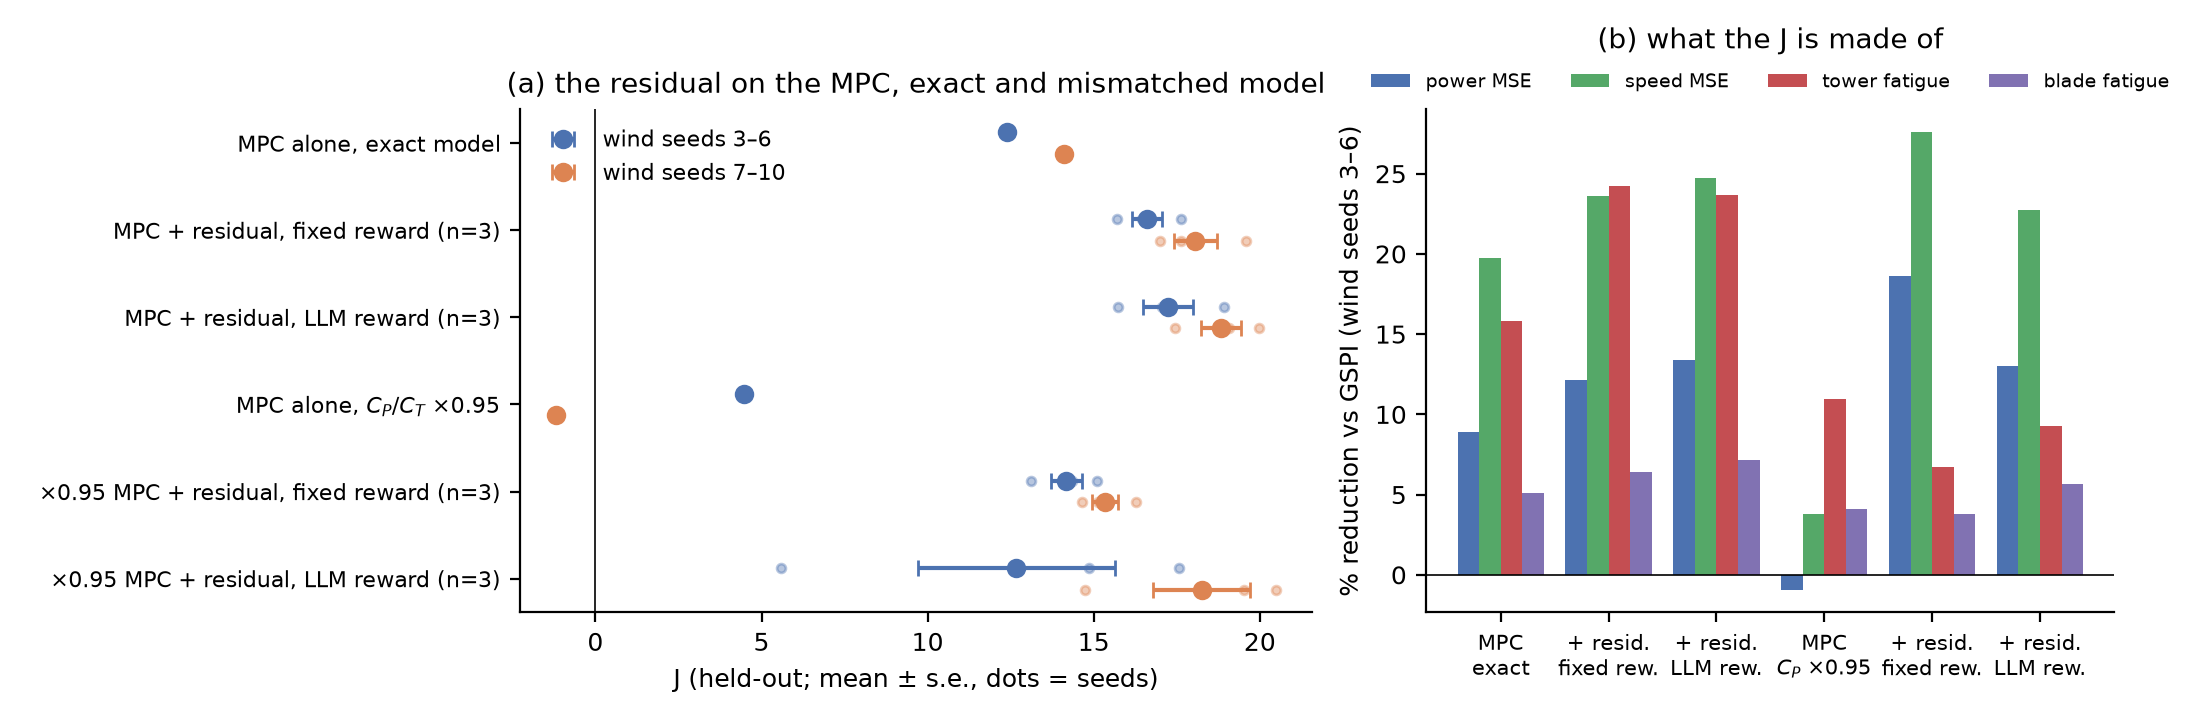
\includegraphics[width=\linewidth]{fig_mpcbase.png}
\caption{Residual on the MPC base. (a) Held-out \J\ on both wind sets for the MPC alone and with the supervised residual, with an exact model and with the power/thrust coefficients 5\,\% low in the MPC's model (mean $\pm$ s.e., dots are seeds). (b) The four terms of \J\ on wind seeds 3--6 for the same rows.}
\label{fig:mpcbase}
\end{figure}

\begin{table}[t]
\centering\small
\caption{The residual on the MPC base (held-out; mean $\pm$ s.d.; composition on wind seeds 3--6 as power MSE / speed MSE / tower fatigue / blade fatigue, \% reduction vs.\ GSPI). Energy is within $\pm0.2$\,\% of GSPI in every row.}
\label{tab:mpcbase}
\resizebox{\linewidth}{!}{%
\begin{tabular}{llcccc}
\toprule
controller & $n$ & \J\ seeds 3--6 & \J\ seeds 7--10 & P\,/\,$\omega$\,/\,T\,/\,B (seeds 3--6) & all four positive \\
\midrule
LPV-MPC alone, exact model                        & --- & 12.40 & 14.10 & 8.9 / 19.8 / 15.8 / 5.1 & yes \\
\textbf{MPC + residual, fixed reward}             & 3 & $16.60\pm0.78$ & $18.06\pm1.10$ & 12.1 / 23.6 / 24.2 / 6.4 & 3/3 \\
\textbf{MPC + residual, LLM-written reward}       & 3 & $17.23\pm1.30$ & $18.84\pm1.04$ & 13.4 / 24.7 / 23.6 / 7.2 & 3/3 \\
\midrule
LPV-MPC alone, $C_P$/$C_T$ $\times0.95$ in its model    & --- & 4.48 & $-1.0$ & $-$1.1 / 3.8 / 11.0 / 4.1 & no \\
\textbf{$\times0.95$ MPC + residual, fixed reward}     & 3 & $14.17\pm0.82$ & $15.35\pm0.68$ & 18.6 / 27.6 / 6.7 / 3.8 & 3/3 \\
\textbf{$\times0.95$ MPC + residual, LLM-written reward} & 3 & $12.66\pm5.13$ & $18.25\pm2.52$ & 13.0 / 22.7 / 9.3 / 5.7 & 3/3 \\
\bottomrule
\end{tabular}}
\end{table}

Table~\ref{tab:mpcbase} and Fig.~\ref{fig:mpcbase} are the main result. On the exact-model MPC the residual adds $+4$ to $+5$ points on both held-out sets in every seed, with every metric improved and the tower-fatigue reduction rising from 16 to 23--25\,\%; the composition is the MPC's, made larger. On the MPC whose power and thrust coefficients are 5\,\% low---alone at 4.5\,/\,$-1$, its regulation lost---the residual restores 13--18, above the exact-model MPC alone: the residual learns the part of the plant the model gets wrong, on the same wind realisations it has never seen. Between a fixed reward and one written by the agent the difference on the MPC base is about one point on the exact model (one seed of the mismatched arm is poor); what the agent contributes to the residual's reward is the subject of the next section.

\subsection{What the agent contributes: a vocabulary, made real by verification}
\label{sec:agent}

\begin{table}[t]
\centering\small
\caption{The supervision study on the GSPI base (held-out \J, mean $\pm$ s.d.; composition on wind seeds 3--6; ``balanced'' counts seeds on which all four metrics improve; paired differences against the tuned fixed reward with wins and exact $p$).}
\label{tab:ablation}
\resizebox{\linewidth}{!}{%
\begin{tabular}{llcccccc}
\toprule
arm & $n$ & \J\ seeds 3--6 & \J\ seeds 7--10 & P\,/\,$\omega$\,/\,T\,/\,B & balanced & $\Delta\J$ vs.\ fixed (wins, exact $p$) \\
\midrule
fixed reward (tuned)                     & 5 & $4.86\pm2.76$ & $5.50\pm2.09$ & 17.4 / 19.0 / $-$17.6 / 0.7 & 0/5 & --- \\
LLM hyper-parameters                     & 3 & $5.26\pm2.39$ & $7.13\pm3.05$ & 17.1 / 20.7 / $-$18.1 / 1.2 & 0/3 & $-0.5$ / $+0.3$ (2/3, 1.0) \\
random hyper-parameters                  & 3 & $4.93\pm2.02$ & $5.96\pm2.17$ & 15.1 / 17.0 / $-$13.2 / 0.8 & 0/3 & $-0.8$ / $-0.9$ (2/3, 1.0) \\
LLM hyper-parameters $+$ reward, one agent & 5 & $6.37\pm2.94$ & $8.65\pm2.60$ & 15.9 / 16.3 / $-$7.6 / 0.9 & 0/5 & $+1.5$ / $+3.2$ (4/5, 0.31 / 0.13) \\
\textbf{LLM reward expression}           & 5 & $5.30\pm4.17$ & $6.04\pm4.28$ & 6.8 / 10.1 / $\mathbf{+1.5}$ / 2.7 & \textbf{3/5} & $+0.4$ / $+0.5$ (3/5, 0.75 / 0.69) \\
LLM reward expression, told $F$, selected by \J & 5 & $7.00\pm2.12$ & $8.33\pm2.38$ & 9.5 / 14.6 / $+0.9$ / 3.0 & 3/5 & $+2.1$ / $+2.8$ (4/5, 0.31 / 0.19) \\
random reward structure, same loop       & 3 & $6.13\pm0.52$ & $7.06\pm1.35$ & 9.5 / 10.5 / $+2.1$ / 2.5 & 1/3 & $+0.4$ / $+0.3$ (2/3, 1/3; $\approx1$) \\
LLM reward expression, single-shot, no loop & 5 & $4.97\pm1.90$ & $6.66\pm2.75$ & 11.6 / 13.3 / $-$5.5 / 0.5 & 1/5 & $+0.1$ / $+1.2$ (2/5, 3/5; $\approx1$) \\
\bottomrule
\end{tabular}}
\end{table}

\begin{figure}[t]
\centering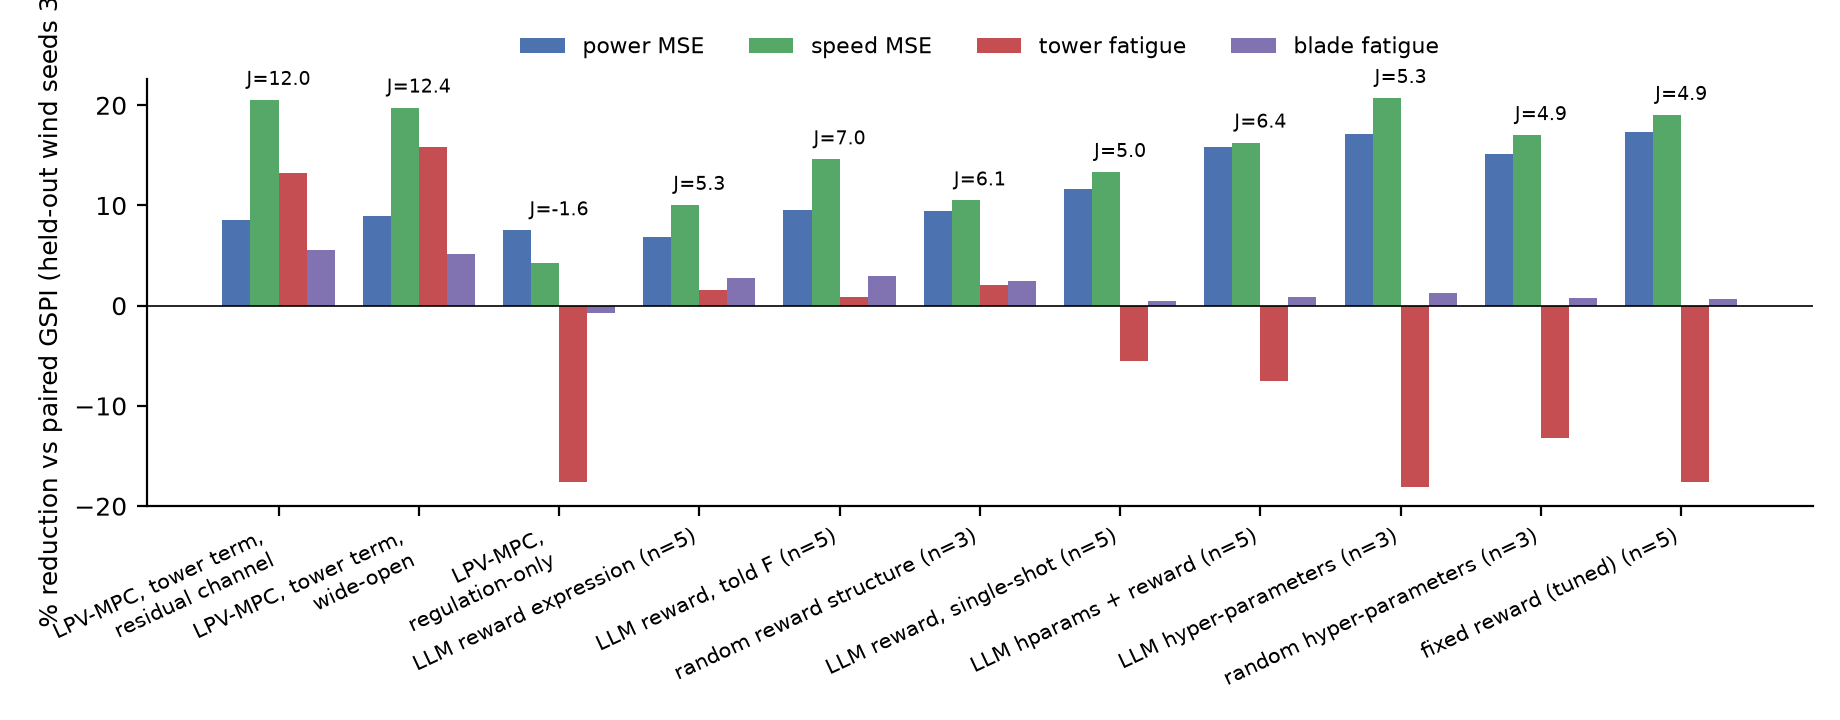
\includegraphics[width=\linewidth]{fig2_composition.png}
\caption{What each controller's \J\ is made of on the GSPI base (held-out wind seeds 3--6, arm means), with the MPC rows for scale. Every fixed-reward and hyper-parameter arm buys regulation with tower fatigue; the reward-expression agent, the random draw from its vocabulary, and the correctly scaled MPC are the rows with every term positive.}
\label{fig:composition}
\end{figure}

On the GSPI base the residual is the whole controller's improvement, so the levers have room to matter; Table~\ref{tab:ablation} and Fig.~\ref{fig:composition} give the outcome, all on the tuned default and both held-out sets.

\paragraph{Numeric levers are worth nothing.} The hyper-parameter agent is worth $-0.5$\,/\,$+0.3$ and random hyper-parameter search $-0.8$\,/\,$-0.9$; the two proposers are indistinguishable and neither moves the fixed reward. The weight search (Appendix~\ref{app:weights}) raises \J\ by about two points over an untuned start and never keeps a candidate with a heavier fatigue weight: fatigue responds over tens of episodes, regulation within one fork, so a 30-episode verification horizon is myopic for that knob (Fig.~\ref{fig:mechanism}b); a sweep of the tower weight confirms the balanced region is not on that axis at all ($\lambda_T=3,10,30$: 1.4, $-2.9$, no learning).

\paragraph{The reward's shape changes the composition, not the level.} Every fixed-reward and hyper-parameter arm buys regulation with tower fatigue ($-13$ to $-18$\,\%), the opposite of what a residual load controller is for. The reward-expression agent is the only arm whose mean tower fatigue improves and the only one with seeds on which all four metrics improve (3/5); its balanced seeds share a \emph{saturated} speed term $\tanh(|\delta\omega|/0.005)$ on the wind-labelled subset and centred, bounded load terms $\tanh(\ell-1)$ that penalise only above-baseline load (Appendix~\ref{app:expressions}). Its effect on the level of \J\ is $+0.4$\,/\,$+0.5$ (3/5, $p=0.75$\,/\,$0.69$)---inside seed noise.

\paragraph{The loop is necessary; the prompt is not.} Told $F$, a load-priority objective, the same agent writes the same shapes and, with \J\ selecting its forks, reaches the balanced solution as often (3/5) with the largest paired gain of any arm ($+2.1$\,/\,$+2.8$, 4/5); its fork records show it choosing between candidates whose $F$ and \J\ disagreed, and \J\ won each time because \J\ selects. Asked once and applied blind, the same agent is the fixed reward (1/5 balanced). Pooled over the two looped arms the balanced solution appears in 6 of 10 seeds, in 1 of 5 without the loop and in 0 of 5 fixed-reward seeds.

\paragraph{The prior is a vocabulary.} A random search over expressions drawn from a fixed grammar of the same term families the agent uses, verified by the same loop, lands where the agent lands: $6.13\pm0.52$\,/\,$7.06\pm1.35$, a positive mean tower fatigue, the balanced solution in 1 of 3 seeds, and the saturated forms kept. Once the vocabulary is written down, verification against the objective finds the balanced solution without an LLM; whether the agent finds it more reliably (6/10 against 1/3) is not separable at these seed counts. Combining the reward lever with the hyper-parameter lever in one agent raises the level ($+1.5$\,/\,$+3.2$, 4/5) but never the composition (0/5 balanced): it buys regulation the way the hyper-parameter arms do.

\section{Design rules}
\begin{enumerate}\setlength\itemsep{2pt}
\item \textbf{Put learning where the model fails.} On the MPC base the residual adds five points and repairs a 5\,\% model error; on the PI base the same residual and the same supervision reach a third of that.
\item \textbf{Put the agent on structural decisions; give numeric ones to random search.} No numeric lever, LLM or random, moved a sound default; the reward's shape did, and a random draw from the agent's vocabulary of shapes does as well. Use the agent to write the grammar, and a verified search to explore it.
\item \textbf{Verification against the true objective is the guarantee; the prompt is not.} The agent told the wrong objective produced the right solution because the loop selected on the true one; the agent without the loop produced the default.
\item \textbf{One lever per agent.} The combined agent gained a little level and lost the composition effect.
\item \textbf{Align the reward's subsets and the cost's scales with the objective before crediting the agent.} A speed term gated on a different subset than the objective's metric (Appendix~\ref{app:gating}) and an MPC cost with terms four orders of magnitude apart each moved the comparison by more than any agent did.
\item \textbf{Report composition and reliability, not only means.} The agent's contribution---a solution class, in a fraction of seeds---is invisible in a table of mean \J.
\end{enumerate}

\section{Limitations}
Seed budgets are three for the MPC-base arms and five for the core PI-base arms; no agentic difference in \J\ is significant, and the MPC-base gains, while consistent in every seed, rest on $n=3$. One plant, one training turbulence intensity, two held-out sets of four realisations. The MPC has no preview, a crude tower-state estimator and a two-second horizon; longer horizons were worse with this linearisation. The residual policy observes the simulator's hub wind where the MPC uses ROSCO's estimate; the model error studied is a scalar scaling of the aerodynamic coefficients, not an identified model. The agent is one reasoning model with one prompt family. An individual-pitch extension of the same supervisor was attempted and did not win on any of its levers; the boundary of the present claims is collective pitch.

\bibliographystyle{unsrtnat}
\bibliography{references}

\appendix

\section{Objective, metrics and the tuned default}
\label{app:weights}
The four metrics of \eqref{eq:J} are computed per episode against the paired GSPI run on the same wind realisation: power MSE and generator-speed MSE relative to rated on the steps where hub wind exceeds rated (the 8\,m/s episodes contribute no regulation term), and damage-equivalent loads of tower-base fore-aft moment and blade-root out-of-plane moment over all episodes. Each episode's reduction is clipped to $\pm100$\,\% before averaging so that a single blown regulation episode cannot own the objective. Energy is the total over all episodes.

The tuned default of \eqref{eq:reward} is the per-knob geometric median of the best checkpoints of a three-seed random-search arm over the six knobs on the GSPI base (fork-verified, \J-selected on wind seeds 1--2): $w_P=220$, $w_\omega=25.2$, $\lambda_T=1$, $\lambda_B=1.31$, residual bounds 0.074\,rad (below rated) and 0.05\,rad (above). That search raised held-out \J\ from $4.60\pm2.38$\,/\,$5.96\pm2.02$ (untuned) to $6.70\pm2.12$\,/\,$7.89\pm2.21$ but never kept a candidate with $\lambda_T>1$ (Fig.~\ref{fig:mechanism}b). The tower-weight sweep from the tuned default (seed 0, wind seeds 3--6\,/\,wind seeds 7--10): $\lambda_T=1$: 5.0\,/\,5.9; 3: 1.4\,/\,3.7; 10: $-2.9$\,/\,$-3.3$; 30: the policy never left its initial state. The same default is used unchanged on the MPC base.

\section{Why the reward's speed term is gated by the wind label}
\label{app:gating}
\begin{figure}[t]
\centering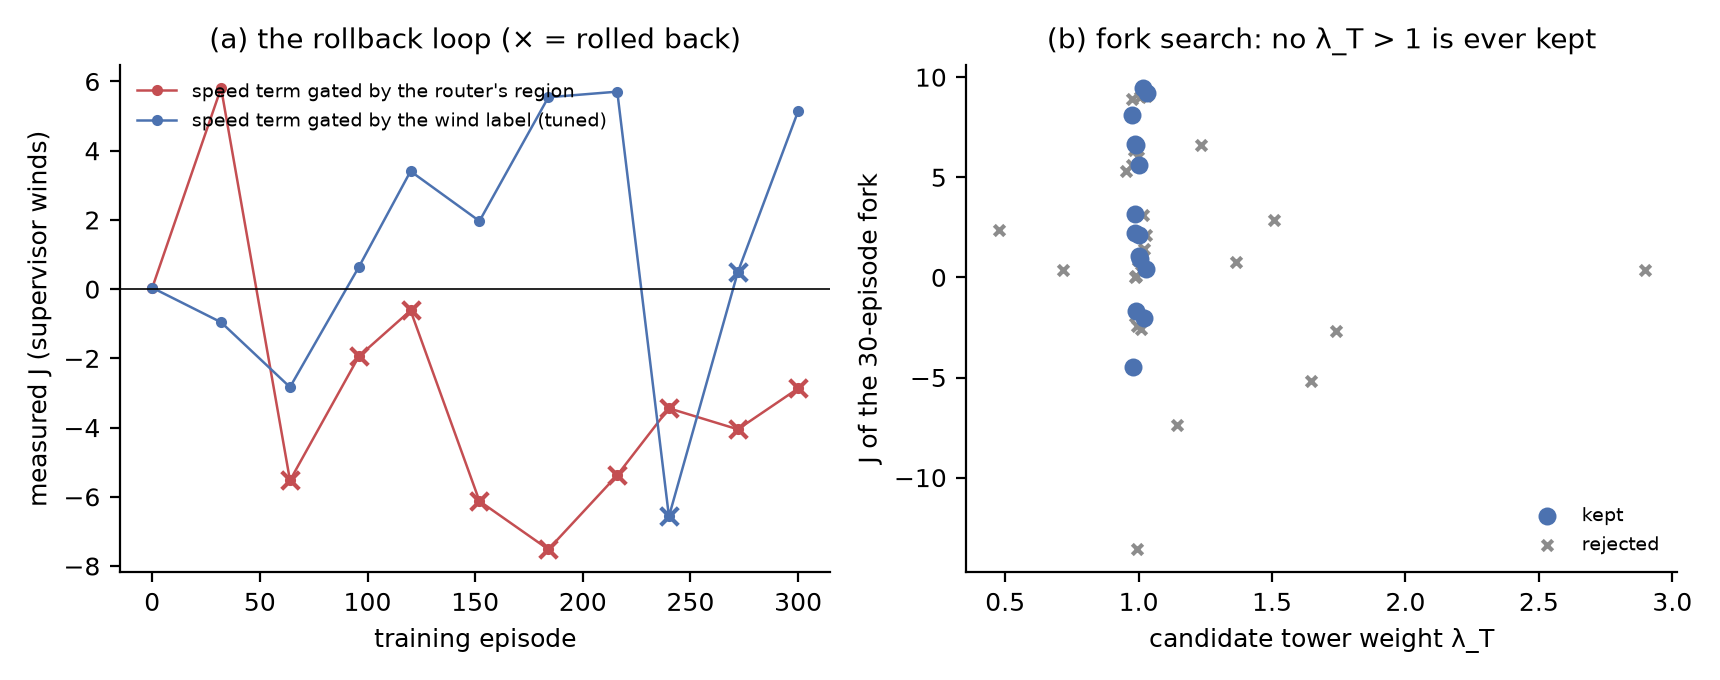
\includegraphics[width=\linewidth]{fig3_mechanism.png}
\caption{(a) Measured \J\ on the supervisor winds at every decision of a fixed-reward run whose speed term is gated by the router's region (red) and of the tuned default gated by the wind label (blue); crosses mark rollbacks. (b) Every fork candidate's tower weight against the \J\ of its 30-episode fork in the weight search; no candidate with $\lambda_T>1$ is ever kept.}
\label{fig:mechanism}
\end{figure}
The objective's regulation metrics are scored on the steps where hub wind exceeds rated, whatever the controller does. If the reward's speed term is instead gated by the router's region, the transition steps at 12.5\,m/s---router ``below rated'', objective ``above''---carry no speed penalty, and the policy is rewarded there for load reduction that the objective scores as regulation loss. Under that gating every fixed-reward run found an early optimum and then rolled back at every later decision (Fig.~\ref{fig:mechanism}a): held-out \J\ $1.59\pm0.87$\,/\,$0.97\pm1.37$ ($n=3$). On that default, hyper-parameter supervision appears valuable ($+5.7$\,/\,$+8.0$ for the LLM, $+5.8$\,/\,$+7.5$ for random search, both by lengthening the credit window, GAE $\lambda$ 0.98$\to$0.995, and slowing the actor). Gating the speed term by the wind label removes the loop without any agent, and on that default the same hyper-parameter arms are worth nothing (\S\ref{sec:agent}). The aligned gating is used throughout the main text; the lesson is design rule~5.

\section{The MPC: cost scaling, selection, authority, robustness}
\label{app:mpc}
The controller model is $J\dot\omega=T_{\mathrm{aero}}(v-\dot x,\omega,\beta)-T_{\mathrm{gen}}(\omega)$, $m\ddot x=F_{\mathrm{thrust}}(v-\dot x,\omega,\beta)-c\dot x-kx$ with the first tower fore-aft mode at 0.324\,Hz, modal mass 437\,t and structural damping ratio 0.01, linearised at the operating point from the $C_P$/$C_T$ tables every 0.1\,s and discretised exactly; tower states are estimated by leaky double integration of the measured nacelle acceleration; the wind input is ROSCO's estimate low-passed at 0.35\,rad/s. The condensed QP over $N=20$ steps minimises
$\sum_k q\,(\delta\omega_k/(0.005\,\omega_{\mathrm{rated}}))^2 + q_t(\dot x_k/0.2)^2 + r\,(\Delta\beta_k/0.002)^2$
subject to the live pitch floor, the pitch limit and the rate limit. Selection on wind seeds 1--2 by \J\ over $N\in\{20,40\}\times r\in\{0.1,0.3,1,3\}\times q_t\in\{0,0.1,0.3,1,3\}\times$ two wind-filter corners (82 points) gives $N=20$, $r=0.3$, $q_t=3$; $N=40$ is worse everywhere. Through the RL's residual channel the same weights are re-selected. Table~\ref{tab:mpc} collects the held-out rows and the model-error study; the model error is applied to the MPC's internal model only.

\begin{table}[h]
\centering\small
\caption{LPV-MPC (\J-selected weights) on the held-out sets and under perturbation of its internal model only.}
\label{tab:mpc}
\resizebox{\linewidth}{!}{%
\begin{tabular}{lcccl}
\toprule
variant & \J\ seeds 3--6 & \J\ seeds 7--10 & P / $\omega$ / T / B (seeds 3--6) & note \\
\midrule
full authority, exact model & 12.40 & 14.10 & 8.9 / 19.8 / 15.8 / 5.1 & base of \S\ref{sec:main} \\
residual channel ($\pm0.05$\,rad, damped), exact model & 11.97 & 11.61 & 8.5 / 20.5 / 13.2 / 5.6 & \\
regulation-only cost ($q_t=0$, unscaled) & $-1.64$ & $-8.08$ & 7.5 / 4.2 / $-$17.6 / $-$0.7 & the published verdict \\
full authority, $C_P$/$C_T$ $\times0.95$ & 4.48 & $-1.0$ & $-$1.1 / 3.8 / 11.0 / 4.1 & base of \S\ref{sec:main} \\
\midrule
residual channel, $C_P$/$C_T$ $\times0.85$ & $-0.37$ & & $-$3.8 / $-$2.8 / 2.6 / 2.5 & regulation lost \\
residual channel, $C_P$/$C_T$ $\times0.95$ & 5.42 & & 1.4 / 7.8 / 8.3 / 4.1 & \\
residual channel, $C_P$/$C_T$ $\times1.05$ & 3.10 & & $-$9.1 / $-$0.1 / 17.0 / 4.5 & \\
residual channel, $C_P$/$C_T$ $\times1.15$ & $-27.53$ & & $-$58.2 / $-$74.2 / 16.5 / 5.7 & regulation collapses \\
residual channel, tower frequency $\times0.9$ / $\times1.1$ & 6.91 / 10.63 & & & \\
residual channel, modal mass $\times0.8$ / $\times1.2$ & 11.00 / 12.22 & & & \\
residual channel, turbulence intensity 14\,\% / 22\,\% (15\,m/s) / 18\,m/s & 10.43 / 12.31 / 22.45 & & & off-design winds \\
\bottomrule
\end{tabular}}
\end{table}

\section{Reward expressions written by the agent}
\label{app:expressions}
Best-checkpoint expressions of the reward-expression agent on the GSPI base (variables: \texttt{region} = router region, \texttt{region\_w} = wind label, \texttt{d\_wg} = relative speed error, \texttt{p\_ratio} = power over paired GSPI power, \texttt{load\_t}, \texttt{load\_b} = fatigue proxies, \texttt{act} = actuation cost). Seed 0, told \J:
\begin{small}\begin{verbatim}
  180*tanh(15*(p_ratio-1))                                    if region==0
  -40*sqrt(tanh(abs(d_wg)/.005)**2 + tanh(60*abs(p_ratio-1))**2)   if region_w==1
  -.9*tanh(log((2+load_t+load_b)/4)) - .1*tanh(act)
\end{verbatim}\end{small}
Seed 1, told $F$:
\begin{small}\begin{verbatim}
  155*tanh(p_ratio-1)                                          if region==0
  -26*tanh(abs(d_wg)/.005)                                     if region_w==1
  -(1.4 if region==0 else .5)*tanh(load_t)
  -(1.0 if region==0 else 1.5)*tanh(load_b) - .1*tanh(act)
\end{verbatim}\end{small}
Seed 0, told $F$:
\begin{small}\begin{verbatim}
  130*tanh(6*(p_ratio-1))*(region==0) - 24*tanh(d_wg/.005)**2*(region_w==1)
  + 1.0*tanh((1-load_t)/(1+load_t)) + 1.1*tanh((1-load_b)/(1+load_b)) - .04*tanh(act)
\end{verbatim}\end{small}
The random structural control samples expressions of the same families with log-uniform coefficients spanning the ranges the agent used. Speed terms, in $x=\delta\omega/0.005$: $x^2$, $|x|$, $\tanh|x|$, $\tanh(x^2)$, $\sqrt{|x|}$. Load terms, in $\ell\in\{\ell_T,\ell_B\}$: $\ell$, $\min(\ell,3)$, $\tanh(\ell-1)$, $\tanh\ell$, $\max(0,\ell-1)$, $\log(1+\ell)$. An optional power-deviation term on the wind-labelled subset.

\section{Paired differences and the full controller list}
\label{app:paired}
\begin{figure}[h]
\centering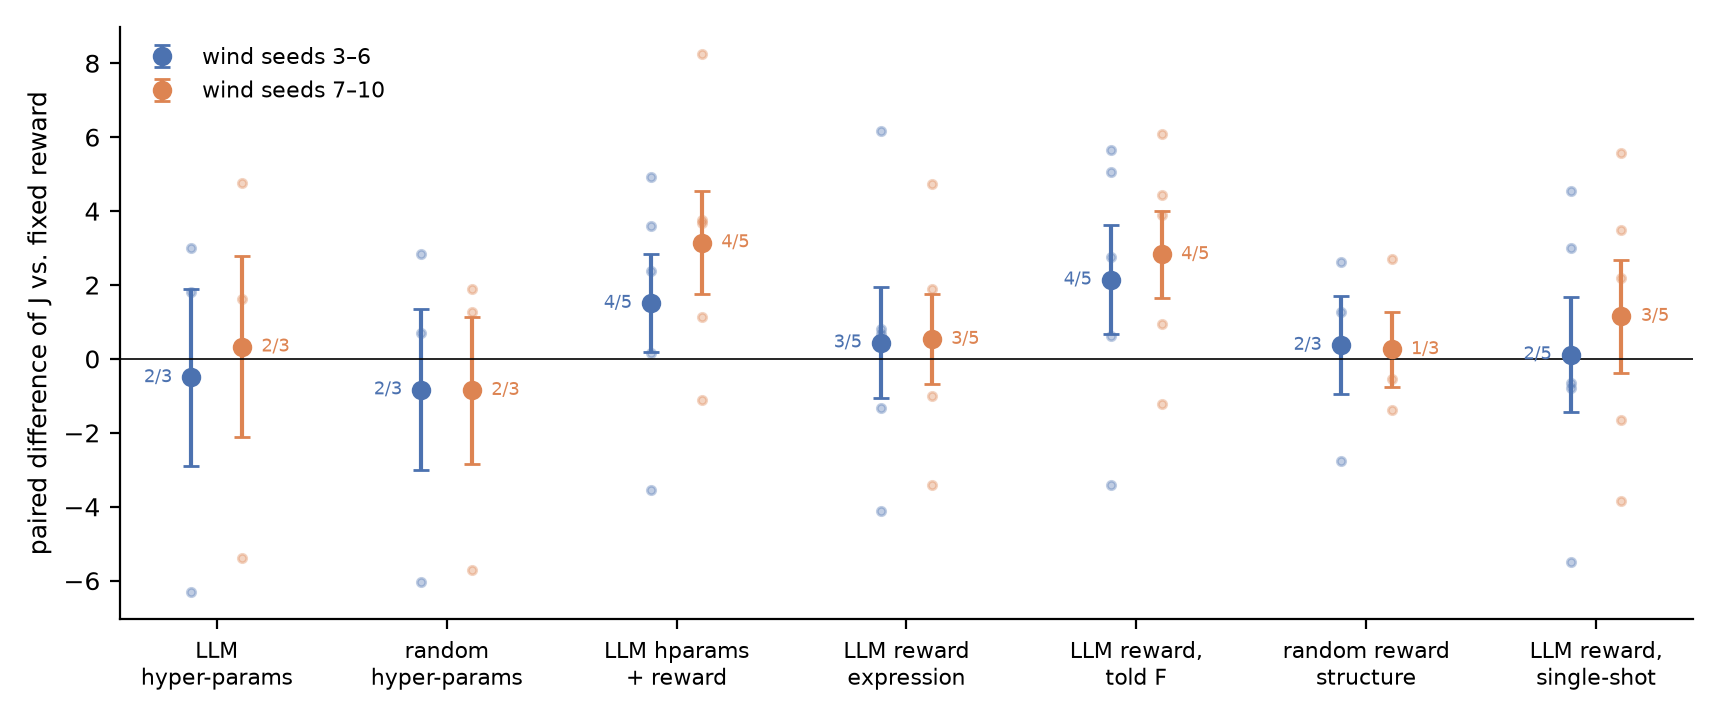
\includegraphics[width=0.85\linewidth]{fig1_levers.png}
\caption{Seed-paired difference of \J\ between each supervised arm and the tuned fixed reward on the GSPI base, both held-out wind sets (mean $\pm$ s.e., dots are seeds, labels are wins$/n$).}
\label{fig:levers}
\end{figure}
\begin{figure}[h]
\centering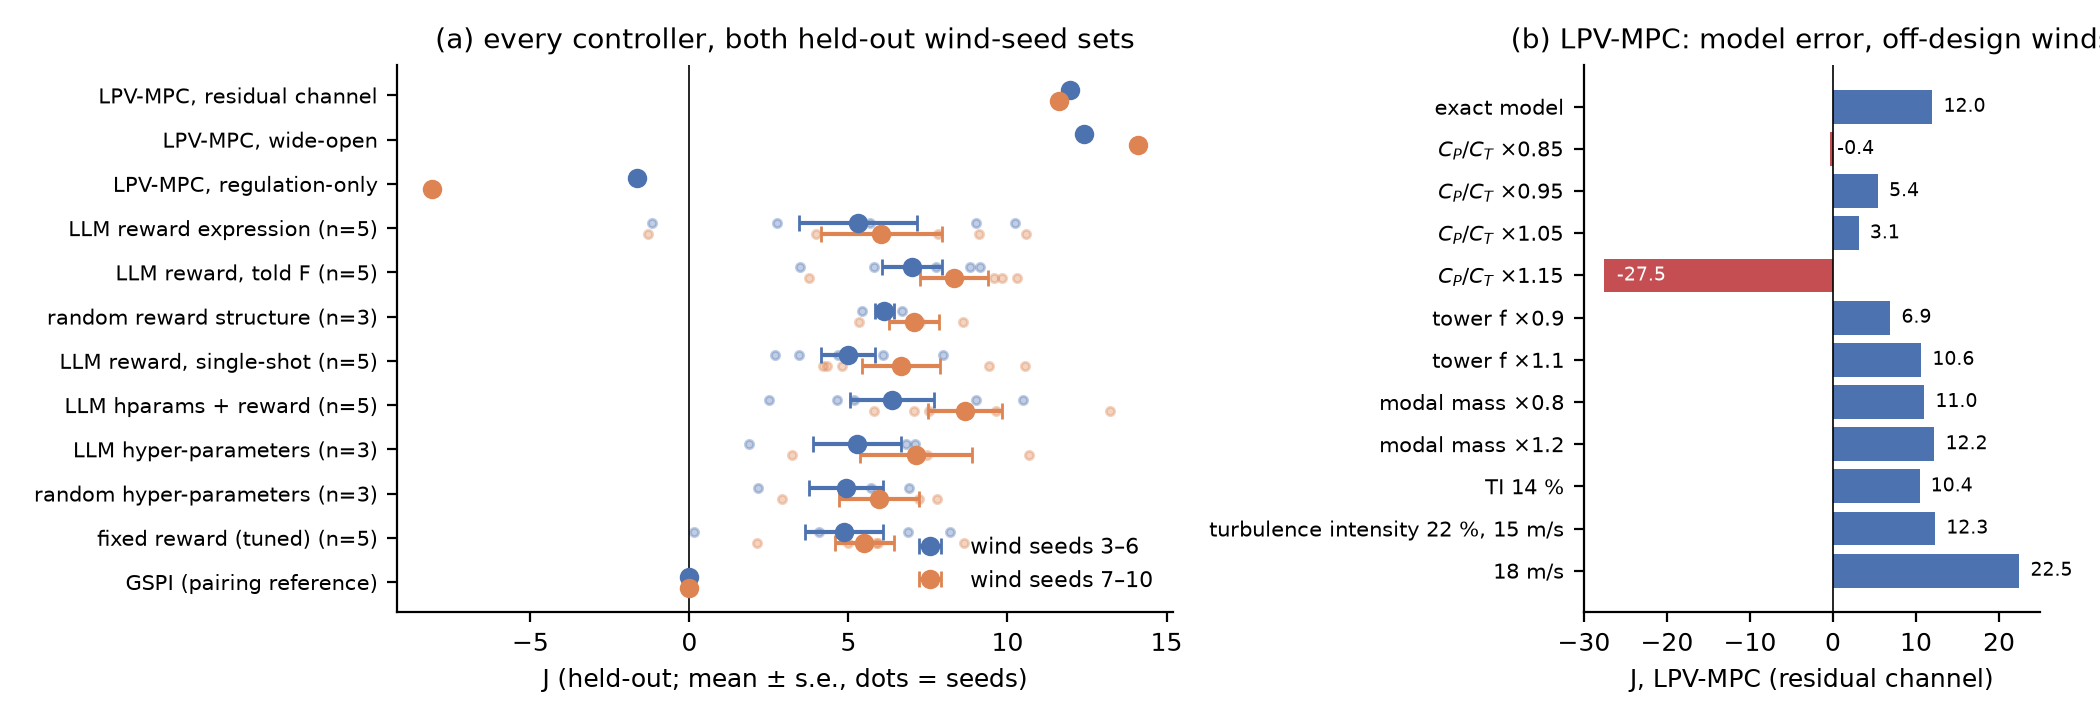
\includegraphics[width=\linewidth]{fig4_reference.png}
\caption{(a) \J\ of every GSPI-base controller and the MPC variants on both held-out sets. (b) The MPC through the residual channel under model error and off-design winds (the data of Fig.~\ref{fig:mpc_error}, with the wind classes).}
\label{fig:reference}
\end{figure}

\section{Compute and reproducibility}
\label{app:compute}
One 300-episode training run takes 65--85 minutes on 16 CPU cores (8 OpenFAST workers, two runs in parallel); the MPC in the worker adds 3.6\,ms per 0.1\,s solve. A supervised run makes about five LLM calls. All runs write rolling checkpoints and can be paused and resumed; every number in this paper is regenerated by the scripts in the repository from the run artefacts, and the figures by a single script.

\end{document}
